% ============================================================
% MS Economics Dissertation — Jawaharlal Nehru University
% ============================================================
\documentclass[12pt,a4paper,oneside]{report}

% ── Fonts & Encoding ──────────────────────────────────────
\usepackage[T1]{fontenc}
\usepackage[utf8]{inputenc}
\usepackage{times}          % Times New Roman body text

% ── Page Layout ───────────────────────────────────────────
% Standard academic dissertation margins
\usepackage[
  top=1in,
  bottom=1in,
  left=1.25in,      % wider left for binding
  right=1in,
  a4paper
]{geometry}

% Line spacing: 1.5 as required by most universities
\usepackage{setspace}
\onehalfspacing

% ── Text Alignment & Paragraph Style ──────────────────────
\setlength{\parindent}{0pt}          % no first-line indent on any paragraph
\setlength{\parskip}{6pt}            % small vertical gap between paragraphs
\raggedbottom                        % don't stretch pages vertically

% ── Graphics ──────────────────────────────────────────────
\usepackage{graphicx}
\graphicspath{{outputs/figures/}{dissertation-report-helpers/}}
\usepackage{float}
\usepackage[
  font=small,          % 10pt captions
  labelfont=bf,        % bold "Figure X.X:" label
  labelsep=period,     % period after number
  justification=justified,
  singlelinecheck=false
]{caption}

% ── Tables ────────────────────────────────────────────────
\usepackage{booktabs}
\usepackage{array}
\usepackage{tabularx}
\usepackage{multirow}
\usepackage{longtable}

% ── Math ──────────────────────────────────────────────────
\usepackage{amsmath,amssymb}

% ── Headers & Footers ─────────────────────────────────────
\usepackage{fancyhdr}
\setlength{\headheight}{15pt}
\pagestyle{fancy}
\fancyhf{}
% Left header: chapter name; Right header: page number
\fancyhead[L]{\small\itshape\nouppercase{\leftmark}}
\fancyhead[R]{\small\thepage}
\renewcommand{\headrulewidth}{0.4pt}
% Plain style (chapter opening pages): page number centred at bottom
\fancypagestyle{plain}{%
  \fancyhf{}%
  \fancyfoot[C]{\small\thepage}%
  \renewcommand{\headrulewidth}{0pt}%
}

% ── Chapter & Section Headings ────────────────────────────
\usepackage{titlesec}

% Chapter: "Chapter 1" on line 1, title on line 2, both centred
% Size: \Large (≈17pt at 12pt base) — slightly larger than body
\titleformat{\chapter}[display]
  {\normalfont\Large\bfseries\centering}
  {\MakeUppercase{\chaptertitlename}\ \thechapter}
  {8pt}
  {\Large}
\titlespacing*{\chapter}{0pt}{-10pt}{24pt}

% Section: 14pt bold, flush left
\titleformat{\section}
  {\normalfont\large\bfseries}
  {\thesection}
  {1em}{}
\titlespacing*{\section}{0pt}{14pt plus 2pt minus 2pt}{6pt}

% Subsection: 12pt bold italic, flush left
\titleformat{\subsection}
  {\normalfont\normalsize\bfseries\itshape}
  {\thesubsection}
  {1em}{}
\titlespacing*{\subsection}{0pt}{10pt plus 2pt minus 2pt}{4pt}

% Subsubsection: 12pt italic, flush left
\titleformat{\subsubsection}
  {\normalfont\normalsize\itshape}
  {\thesubsubsection}
  {1em}{}
\titlespacing*{\subsubsection}{0pt}{8pt}{2pt}

% ── Hyperlinks ────────────────────────────────────────────
\usepackage[hidelinks,hypertexnames=false]{hyperref}
\usepackage{bookmark}

% ── Miscellaneous ─────────────────────────────────────────
\usepackage{enumitem}
\usepackage{url}
\urlstyle{same}                       % URL in same font as body
\newcommand{\citep}[1]{\cite{#1}}

\begin{document}

% ============================================================
%  TITLE PAGE
% ============================================================
\begin{titlepage}
\begin{center}

\vspace*{0.8cm}

{\LARGE \textbf{Do Global Oil Price Shocks Raise\\[6pt]
India's Inflation More Than\\[6pt]
They Lower It?}}

\vspace{0.6cm}

{\large \textit{Short-Run Pass-Through to CPI Inflation\\in India, 2004--2024}}

\vspace{0.8cm}

{\large Dissertation submitted for the degree of\\[4pt]
\textit{Master of Science (Economics)}}

\vspace{0.8cm}

{\large \textbf{Aniket Pandey}}

\vspace{1cm}


\includegraphics[width=3.5cm]{jnu-logo.png}

\vfill

{\large \textbf{Centre for Economic Studies and Planning}\\[4pt]
\textbf{School of Social Sciences}\\[4pt]
\textbf{Jawaharlal Nehru University}\\[4pt]
\textbf{New Delhi}\\[4pt]
\textbf{India}\\[4pt]
\textbf{2026}}

\end{center}
\end{titlepage}

\cleardoublepage

% ============================================================
%  CERTIFICATE PAGE
% ============================================================
\thispagestyle{empty}
\setcounter{page}{0}

% --- Compact letterhead header ---
\noindent
\begin{minipage}[c]{0.18\textwidth}
  
\includegraphics[width=2cm]{jnu-logo.png}
\end{minipage}%
\hfill
\begin{minipage}[c]{0.78\textwidth}
  \raggedright
  {\small\textbf{Centre for Economic Studies and Planning}}\\[-1pt]
  {\small\textbf{School of Social Sciences, Jawaharlal Nehru University}}\\[-1pt]
  {\small\textbf{New Delhi--110067, India}}
\end{minipage}

\vspace{0.4cm}
\noindent\rule{\textwidth}{0.8pt}
\vspace{0.6cm}

\begin{center}
{\LARGE \textbf{CERTIFICATE}}
\end{center}

\vspace{0.8cm}

\noindent This is to certify that the dissertation titled ``\textbf{Do Global Oil Price Shocks Raise India's Inflation More Than They Lower It? Short-Run Pass-Through to CPI Inflation in India, 2004--2024}'' submitted by \textbf{ANIKET PANDEY}, in partial fulfillment of the requirements for the award of the degree of \textbf{Master of Science (Economics)} at the Centre for Economic Studies and Planning, School of Social Sciences, Jawaharlal Nehru University, New Delhi, has not been previously submitted in part or in full for any other degree of this university or any other university/institution.

\vspace{0.8cm}

\noindent We recommend this dissertation be placed before the examiners for evaluation for the award of the degree of M.Sc.\ Economics.

\vspace{3cm}

\noindent
\begin{minipage}[t]{0.45\textwidth}
\textbf{Prof.\ Shakti Kumar}\\
SUPERVISOR
\end{minipage}
\hfill
\begin{minipage}[t]{0.45\textwidth}
\raggedleft
\textbf{Chairperson}\\
CHAIRPERSON
\end{minipage}

\newpage

% ============================================================
%  ACKNOWLEDGEMENTS
% ============================================================
\thispagestyle{empty}
\begin{center}
{\LARGE \textbf{Acknowledgements}}
\end{center}
\vspace{1cm}

\noindent I owe a great deal to Prof.\ Shakti Kumar, whose guidance shaped this dissertation from start to finish. His willingness to discuss methodology at length, correct my mistakes, and push me toward honest interpretation made the final product far better than anything I could have managed alone.

I am also grateful to the faculty at the Centre for Economic Studies and Planning for two years of rigorous coursework that gave me the econometric tools needed for this study. The library staff at JNU and the creators of the FRED and MoSPI data portals deserve thanks for making high-quality economic data freely accessible.

My classmates, especially those who sat through early presentations of this work and offered blunt feedback, improved it considerably. Finally, I thank my family for their patience during the months when this dissertation consumed most of my attention.

\vspace{1cm}
\begin{flushright}
Aniket Pandey\\
New Delhi, 2026
\end{flushright}

\newpage

% ============================================================
%  ABSTRACT
% ============================================================
\thispagestyle{empty}
\begin{center}
{\LARGE \textbf{Abstract}}
\end{center}
\vspace{1cm}

\noindent India imports roughly 85 per cent of its crude oil, which makes domestic inflation sensitive to global oil price movements. This dissertation asks whether positive oil price shocks raise India's consumer price inflation by more than negative shocks lower it, a pattern known in the literature as ``rockets and feathers'' asymmetry.

Using monthly data from April 2004 to December 2024, I estimate an asymmetric autoregressive distributed lag model in first differences, with Brent crude oil prices converted to Indian rupees as the main oil price variable. The autoregressive lag order is selected by AIC, and all inference uses Newey--West heteroskedasticity and autocorrelation consistent standard errors.

The main finding is that positive oil shocks are associated with higher monthly CPI inflation, with a cumulative pass-through coefficient of 0.021. A 10 per cent increase in rupee-denominated oil prices raises monthly inflation by about 0.21 percentage points. The corresponding estimate for negative oil shocks is near zero. However, a Wald test for the equality of positive and negative cumulative pass-through fails to reject symmetry at the 5 per cent level ($p = 0.24$). This means the point estimates suggest asymmetric behaviour, but the statistical evidence is not strong enough to confirm it in headline CPI.

Robustness checks that separate the Brent price from the exchange rate show a stronger and marginally significant positive pass-through. An appendix analysis using the official Fuel and Light CPI sub-index, which is more directly exposed to energy costs, produces a larger and statistically significant positive oil pass-through ($p = 0.03$). These results together indicate that oil prices do matter for Indian inflation, even though the asymmetry is hard to pin down precisely at the aggregate level.

\textbf{Keywords:} Oil price pass-through, CPI inflation, asymmetric adjustment, India, autoregressive distributed lag model, Newey--West inference

\newpage

% ============================================================
%  TABLE OF CONTENTS, LIST OF TABLES, LIST OF FIGURES
% ============================================================
\pagenumbering{roman}
\setcounter{page}{1}
\tableofcontents
\newpage
\listoftables
\newpage
\listoffigures
\newpage

% ============================================================
%  MAIN TEXT BEGINS
% ============================================================
\pagenumbering{arabic}

% placeholder for chapters
\chapter{Introduction}
\label{ch:introduction}

India is the world's third-largest consumer of crude oil and imports roughly 85 per cent of its requirements. This dependence means that movements in global oil prices feed directly into domestic costs, affecting everything from transport and manufacturing to household cooking fuel. When global oil prices rise, the cost of imported crude increases India's import bill, puts downward pressure on the rupee, and raises input costs across sectors. The resulting inflationary pressure concerns policymakers at the Reserve Bank of India (RBI), which targets a 4 per cent headline CPI inflation rate under its flexible inflation targeting framework.

A natural question follows: does a fall in oil prices bring inflation down by just as much as a rise pushes it up? The answer matters for monetary policy, fiscal planning, and welfare. If oil price increases pass through to consumer prices more strongly than decreases, a pattern the literature calls ``rockets and feathers,'' then the average inflationary effect of oil price volatility is positive, even when oil prices fluctuate symmetrically around their mean. Households would bear a net inflationary cost from oil price instability, and the central bank would need to account for this asymmetry in its inflation forecasts.

\section{Research Question}

This dissertation examines the short-run pass-through of global oil price shocks to India's headline CPI inflation over the period April 2004 to December 2024. Two specific questions guide the analysis:

\begin{enumerate}[label=(\roman*)]
\item Do positive oil price shocks raise monthly CPI inflation by an economically meaningful amount?
\item Is the pass-through from oil price increases larger than that from oil price decreases?
\end{enumerate}

The first question asks whether oil prices matter for Indian inflation in the short run. The second asks whether the transmission is asymmetric.

\section{Motivation}

Several features of India's economy make this question worth studying in detail.

First, India's fuel pricing regime has changed considerably during the sample period. Petrol prices were formally deregulated in June 2010, and diesel prices followed in October 2014. Before deregulation, the government absorbed much of the oil price volatility through subsidies, which may have dampened pass-through to consumer prices. After deregulation, domestic retail fuel prices began tracking international prices more closely, at least in principle. This institutional change provides a natural setting for comparing pass-through across two distinct policy regimes.

Second, the exchange rate adds a layer of complexity that is specific to India's situation. India pays for crude oil in US dollars, so a depreciation of the rupee against the dollar amplifies the domestic-currency cost of any given oil price increase. This means that India-specific inflationary episodes can arise even during periods of stable global oil prices, if the rupee weakens. Separating the oil price channel from the exchange rate channel requires explicit attention, which the robustness analysis in this dissertation provides.

Third, India's CPI basket assigns roughly 46 per cent weight to food items and only about 7 per cent directly to fuel and light. This composition means that headline CPI is a noisy measure of energy cost pass-through. Oil prices affect headline CPI through multiple channels (direct fuel costs, transport costs embedded in food distribution, and manufacturing input costs), but the signal gets diluted by weather-driven food inflation and other shocks that have nothing to do with oil. This makes it difficult to obtain precise estimates of oil pass-through in headline CPI, a difficulty that should be acknowledged upfront rather than glossed over.

\section{Approach}

The main empirical model is an asymmetric autoregressive distributed lag (ADL) specification in first differences. Oil price changes are split into positive and negative components, and the cumulative effects of each are estimated separately. The oil lag length is fixed at three months, and the autoregressive CPI lag order is selected by the Akaike information criterion over one to four lags on a common estimation sample. All hypothesis tests use Newey--West heteroskedasticity and autocorrelation consistent (HAC) standard errors, so the inference is robust to serial correlation and heteroskedasticity in the residuals.

For robustness, a separate specification replaces the composite rupee oil price with Brent crude in US dollars and includes the exchange rate as a separate regressor. This allows the world oil price effect and the exchange rate effect to be estimated independently. An appendix extends the analysis to the official CPI Fuel and Light sub-index, which is more directly exposed to energy cost movements than headline CPI.

\section{Structure of the Dissertation}

Chapter 2 reviews the relevant literature on oil price shocks, inflation, and asymmetric pass-through. Chapter 3 describes the data and econometric methodology. Chapter 4 presents the main empirical results, including unit root tests, the baseline symmetric model, the main asymmetric model, and sub-sample comparisons. Chapter 5 covers robustness checks. Chapter 6 discusses the findings and their policy relevance. Chapter 7 concludes.

\chapter{Literature Review}
\label{ch:literature}

\section{Oil Prices and Macroeconomic Performance}

The modern literature on oil shocks and macroeconomics begins with Hamilton (1983), who showed that most US recessions since World War II were preceded by increases in the price of crude oil. That finding prompted a large body of work examining the channels through which oil prices affect output, employment, and inflation. Early studies treated oil shocks as straightforward supply-side events: higher energy costs raise production costs, squeeze profit margins, and push up the general price level. This supply-side mechanism is intuitive and remains a standard feature of macroeconomic textbooks.

By the mid-1990s, a more nuanced picture had emerged. Mork (1989) split oil price changes into positive and negative movements and found that oil price increases depressed US GDP growth, but oil price decreases did not produce a symmetric expansion. Lee, Ni and Ratti (1995) reinforced this finding by showing that oil price volatility conditions mattered: a price increase that comes during a period of stability has more macroeconomic impact than the same increase during a volatile period. Hamilton (2003) formalised various nonlinear measures of oil shocks and argued that the net oil price increase specification better captures the recessionary effects of oil in the US. These studies established asymmetry as a central theme in oil shock research.

On the inflation side, the initial empirical consensus was clear: oil price increases raised inflation. But Hooker (2002) challenged this consensus by showing that the oil--inflation relationship weakened after 1980 in the United States. He attributed this to improved monetary policy credibility, which anchored inflation expectations and prevented oil price increases from generating persistent inflationary spirals. Blanchard and Gal\'{i} (2009) provided additional evidence across developed economies, documenting a decline in the pass-through of oil shocks to both inflation and output since the mid-1980s.

\section{Asymmetric Pass-Through: Rockets and Feathers}

The idea that prices respond faster to cost increases than cost decreases originates in Bacon's (1991) study of UK petrol markets, which gave rise to the ``rockets and feathers'' label. The intuition is straightforward: firms raise output prices quickly when input costs rise, but lower them slowly, or not at all, when costs fall. The pattern has been documented in retail fuel markets across many countries, though the evidence is not unanimous.

At the macroeconomic level, asymmetry in the oil--inflation relationship has been studied using various econometric approaches. Lardic and Mignon (2008) used asymmetric cointegration techniques to study oil price effects in G7 economies and found evidence that the long-run relationship between oil prices and GDP differed depending on the sign of the oil price change. Shin, Yu and Greenwood-Nimmo (2014) developed the nonlinear autoregressive distributed lag (NARDL) framework, which decomposes a regressor into positive and negative partial sum components within a cointegrating equation. Their approach has become popular in applied work because it provides a test for long-run asymmetry within a single-equation error correction framework.

However, not all studies support the asymmetry hypothesis. Kilian and Vigfusson (2011) argued that much of the evidence for asymmetric macroeconomic effects of oil shocks is based on censored regressions that introduce a pre-test bias. Using properly specified models and US data, they found that the evidence for asymmetric effects on GDP was weaker than commonly believed. This critique is relevant for inflation pass-through studies as well, because the same statistical issues apply when oil price changes are split into positive and negative components.

\section{Oil Pass-Through in Emerging Economies}

The pass-through literature is heavily concentrated on developed economies, particularly the United States and Europe. Emerging economies, however, face different conditions that may amplify or dampen oil pass-through. Higher energy intensity of GDP, larger shares of food in consumption baskets, more volatile exchange rates, and fuel price regulation all affect how oil shocks transmit to consumer prices.

Chen (2009) studied oil price pass-through to inflation across 19 industrialised countries and found considerable cross-country variation. Countries with less credible monetary policy and more rigid labour markets tended to exhibit stronger pass-through. For developing countries, the evidence is thinner but growing. Several studies have used vector autoregression and structural approaches to estimate oil price effects, but results vary considerably depending on the time period, the oil price measure, and the identification strategy.

\section{India-Specific Studies}

India's case is particularly interesting because of its high oil import dependence and its history of administered fuel pricing. Bhanumurthy, Das and Bose (2012) examined the macroeconomic effects of oil price shocks on India using a macroeconometric model and found that oil price increases raised inflation and widened the current account deficit. However, they noted that the government's pricing policy at the time, which involved substantial fuel subsidies, significantly dampened the pass-through.

Abu-Bakar and Masih (2018) applied the NARDL framework to India and found evidence of asymmetric oil price pass-through to inflation. Their study covered a period when fuel pricing was partly regulated, and they argued that the asymmetry arose because the government was quicker to raise retail prices when crude prices went up than to lower them when crude prices fell. This is a plausible mechanism, though it is harder to document precisely at the monthly frequency.

Pradeep (2022) studied the effect of diesel price deregulation on the asymmetry of oil price pass-through in India. Using a nonlinear ARDL approach, Pradeep found that deregulation made the pass-through more symmetric in the post-reform period, because retail prices began tracking international prices in both directions. This finding has direct relevance for the present study, because the sample period here covers both the pre-deregulation and post-deregulation regimes.

The Reserve Bank of India itself has examined the oil--inflation link in its Monetary Policy Reports. The RBI has consistently noted that crude oil prices are a key source of inflation risk, particularly through their effect on transport costs and the prices of oil-intensive manufactured goods. The RBI's own estimates suggest that a 10 per cent increase in crude oil prices raises headline CPI inflation by about 0.3--0.4 percentage points over a one-year horizon, though this estimate includes both direct and indirect effects.

\section{The Exchange Rate Channel}

A feature of oil pass-through in India that deserves separate attention is the exchange rate. Since India buys oil in US dollars, the rupee--dollar exchange rate mediates the domestic-currency cost of imported crude. A rise in global oil prices combined with a weakening rupee compounds the inflationary impact. Conversely, a fall in oil prices may not fully reduce domestic fuel costs if the rupee depreciates simultaneously.

This dual channel, oil prices in dollars and the exchange rate, means that studies using a composite rupee oil price may conflate two distinct sources of inflationary pressure. If the rupee depreciates for reasons unrelated to oil (such as capital outflows or a widening current account deficit), the composite oil price will show a ``shock'' that is really an exchange rate event. Separating the Brent price in dollars from the exchange rate, as the robustness analysis in this dissertation does, provides a cleaner identification of each channel.

\section{Gaps in the Literature}

Several gaps motivate this dissertation. First, most India studies use data that stop before the full effect of diesel deregulation can be observed. This study extends the sample to December 2024, providing a long post-deregulation window. Second, many studies apply the NARDL or SVAR framework without checking whether simpler reduced-form models deliver similar conclusions. This study uses a transparent ADL framework in first differences, which is easier to interpret and less sensitive to cointegration rank assumptions. Third, few India studies explicitly separate the oil price channel from the exchange rate channel with both reported in the same specification. The Brent-plus-exchange-rate robustness model in this study addresses that gap. Fourth, using the sub-index for Fuel and Light CPI from the official MoSPI data provides a direct check on whether the dilution effect in headline CPI obscures the true pass-through.

\chapter{Data and Methodology}
\label{ch:data}

\section{Data Sources and Sample Period}

The study uses monthly data from April 2004 to December 2024, giving 249 observations before differencing and a usable estimation sample of approximately 245 observations after accounting for lagged variables. Four data series are used:

\begin{table}[H]
\centering
\caption{Data Sources and Description}
\label{tab:data_sources}
\begin{tabular}{llll}
\toprule
\textbf{Variable} & \textbf{Description} & \textbf{Source} & \textbf{Unit} \\
\midrule
CPI & Headline Consumer Price Index & OECD via FRED & Index (2015=100) \\
Brent & Brent crude oil price & IMF via FRED & USD per barrel \\
EXR & INR/USD exchange rate & Federal Reserve via FRED & Rupees per USD \\
IIP & Index of Industrial Production & RBI DBIE & Chain-linked index \\
\bottomrule
\end{tabular}
\end{table}

The CPI series is the all-items consumer price index for India from the OECD's Main Economic Indicators database, accessed through the Federal Reserve Bank of St.\ Louis (FRED). The Brent crude oil price is the average monthly spot price reported by the IMF, also obtained through FRED. The INR/USD exchange rate is the monthly average from the Federal Reserve. The IIP data come from the Reserve Bank of India's Database on Indian Economy (DBIE) and are chain-linked to provide a consistent monthly activity measure across different base years.

The sample starts in April 2004 because this is the earliest month for which all four series overlap reliably. The choice of end date at December 2024 allows the analysis to capture the full post-diesel-deregulation period (October 2014 onward), the COVID-19 disruption, and the oil price spike associated with the Russia--Ukraine conflict in 2022.

Figure~\ref{fig:raw_series} shows the four raw series in levels. CPI has a clear upward trend, reflecting India's persistent positive inflation over the sample period. Brent crude shows large swings, including the collapse during the 2008--09 financial crisis, the 2014--16 decline, and the COVID-19 crash in early 2020. The exchange rate depreciates steadily from about 40 rupees per dollar in 2004 to about 85 by the end of 2024. The IIP index shows a broadly upward trend with pronounced seasonal variation and a sharp drop during the COVID lockdown.

\begin{figure}[H]
\centering
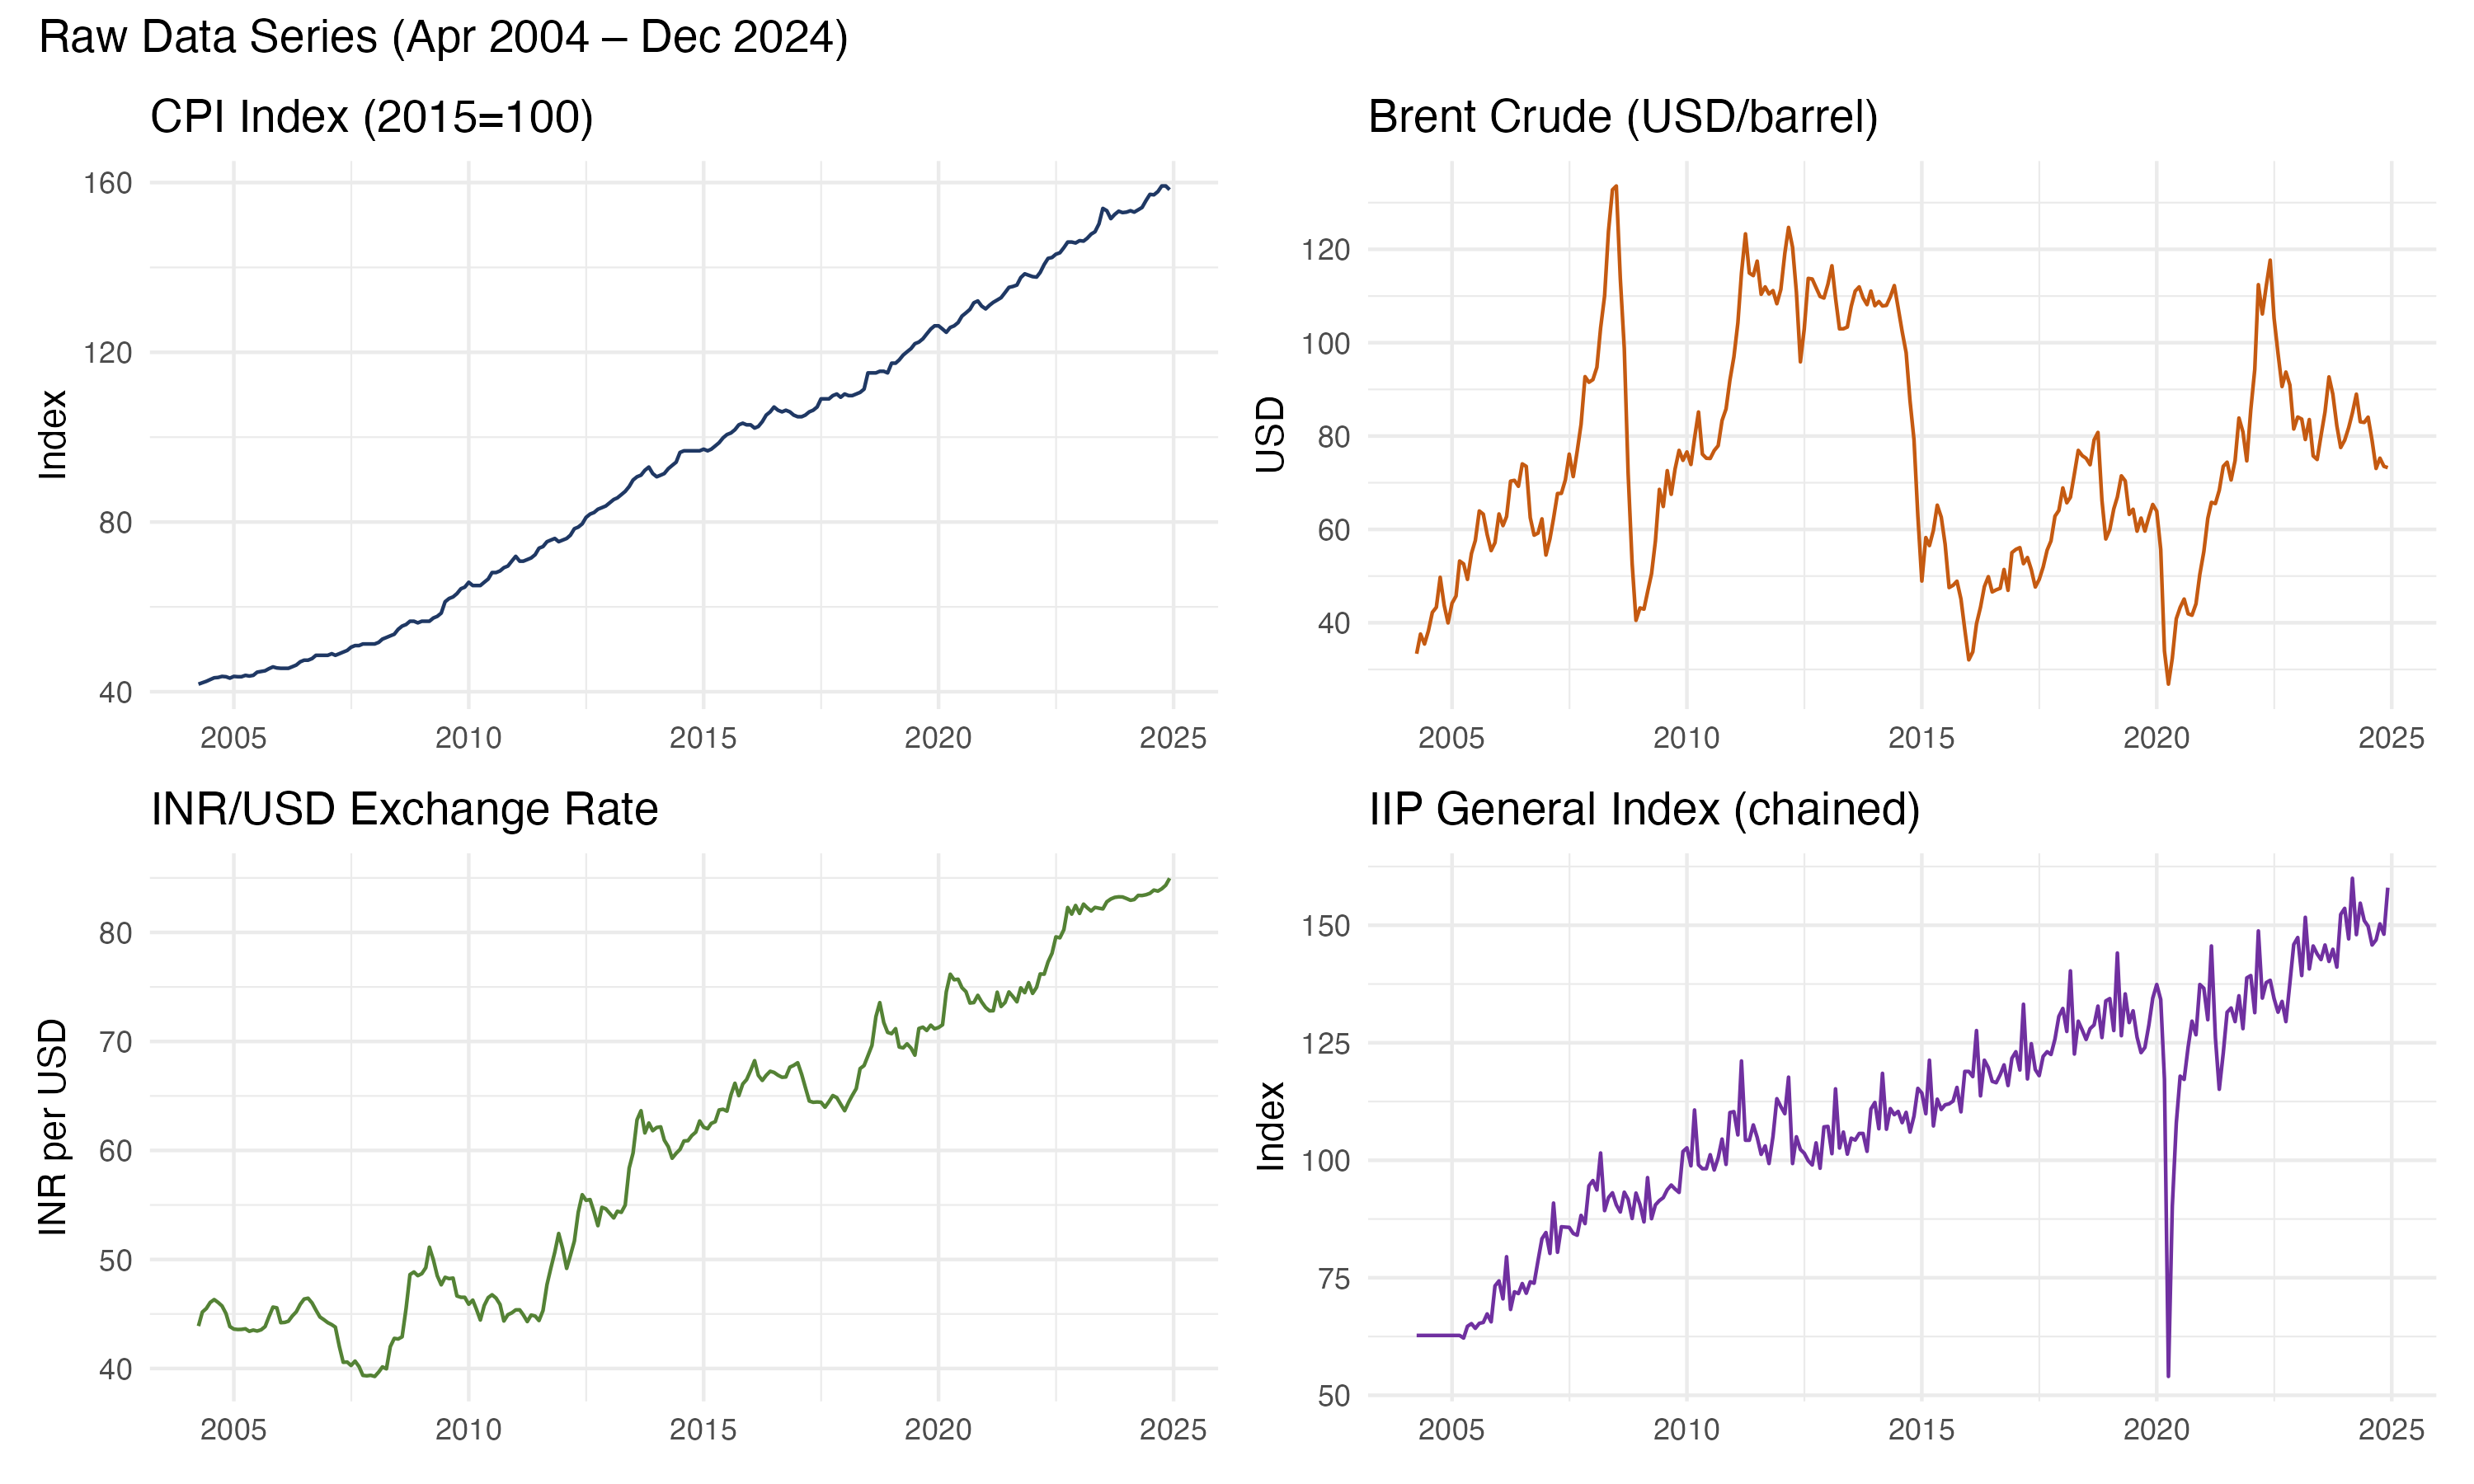
\includegraphics[width=0.95\textwidth]{fig_1_raw_series.png}
\caption[Raw Data Series in Levels, 2004--2024]{}
\label{fig:raw_series}
\end{figure}

\section{Variable Construction}

From the raw data, a composite rupee-denominated oil price is constructed as:
\begin{equation}
\text{Oil\_INR}_t = \text{Brent\_USD}_t \times \text{EXR}_t
\label{eq:oil_inr}
\end{equation}

This composite price reflects the actual cost of imported crude in Indian rupees. All series are then converted to monthly log-differences, expressed as percentages:
\begin{equation}
\Delta \ln X_t = 100 \times [\ln(X_t) - \ln(X_{t-1})]
\label{eq:logdiff}
\end{equation}

where $X$ is CPI, Oil\_INR, EXR, IIP, or Brent. The resulting variables, $\Delta \ln \text{CPI}_t$, $\Delta \ln \text{Oil}_t$, $\Delta \ln \text{EXR}_t$, and $\Delta \ln \text{IIP}_t$, represent approximate percentage changes and are stationary by construction.

The asymmetric decomposition splits oil price changes into positive and negative components:
\begin{align}
\Delta \ln \text{Oil}^+_t &= \max(\Delta \ln \text{Oil}_t, 0) \label{eq:oilpos} \\
\Delta \ln \text{Oil}^-_t &= \min(\Delta \ln \text{Oil}_t, 0) \label{eq:oilneg}
\end{align}

The negative component is kept negative (not in absolute value). This convention matters for interpreting the coefficients correctly: a positive coefficient on $\Delta \ln \text{Oil}^-_t$ means that oil price decreases are associated with higher inflation (a perverse response), while a negative coefficient means decreases lower inflation as expected.

Figure~\ref{fig:logdiff} shows the log-differenced series, and Figure~\ref{fig:oil_decomp} shows the cumulative partial sums of positive and negative oil price changes.

\begin{figure}[H]
\centering

\includegraphics[width=0.95\textwidth]{fig_2_log_diff_series.png}
\caption[Log-Differenced Series (Monthly Percentage Changes)]{}
\label{fig:logdiff}
\end{figure}

\begin{figure}[H]
\centering

\includegraphics[width=0.85\textwidth]{fig_3_oil_decomposition.png}
\caption[Cumulative Partial Sums of Positive and Negative Oil Price Changes]{}
\label{fig:oil_decomp}
\end{figure}

Table~\ref{tab:desc_stats} reports descriptive statistics for all variables. Monthly CPI inflation averages 0.54 per cent with a standard deviation of 0.75. Oil price changes are much more volatile, with a standard deviation of 8.89 percentage points and a range from $-45.4$ to $+23.2$ per cent. The positive oil component averages 3.60 per cent per month when non-zero, while the negative component averages $-3.02$ per cent.

\begin{table}[H]
\centering
\caption{Descriptive Statistics}
\label{tab:desc_stats}
\begin{tabular}{lrrrrr}
\toprule
\textbf{Variable} & \textbf{N} & \textbf{Mean} & \textbf{SD} & \textbf{Min} & \textbf{Max} \\
\midrule
CPI Index & 249 & 93.97 & 35.71 & 41.79 & 159.20 \\
Brent USD & 249 & 75.08 & 24.26 & 26.85 & 133.59 \\
INR/USD & 249 & 60.21 & 13.89 & 39.27 & 84.97 \\
IIP Index & 249 & 109.97 & 24.46 & 54.00 & 160.00 \\
Oil INR & 249 & 4490.59 & 1692.95 & 1464.13 & 9190.63 \\
$\Delta\ln$CPI (\%) & 248 & 0.54 & 0.75 & $-1.66$ & 4.47 \\
$\Delta\ln$Oil (\%) & 248 & 0.58 & 8.89 & $-45.37$ & 23.20 \\
$\Delta\ln$EXR (\%) & 248 & 0.27 & 1.67 & $-4.14$ & 6.56 \\
$\Delta\ln$IIP (\%) & 248 & 0.37 & 8.28 & $-77.49$ & 51.30 \\
$\Delta$Oil$^+$ (\%) & 248 & 3.60 & 4.58 & 0.00 & 23.20 \\
$\Delta$Oil$^-$ (\%) & 248 & $-3.02$ & 6.02 & $-45.37$ & 0.00 \\
\bottomrule
\end{tabular}
\end{table}

\section{Policy and Event Controls}

Three dummy variables control for known structural and outlier events:

\begin{itemize}
\item $D_{\text{petrol}} = 1$ from June 2010 onward, capturing petrol price deregulation.
\item $D_{\text{diesel}} = 1$ from October 2014 onward, capturing diesel price deregulation.
\item $D_{\text{covid}} = 1$ for April 2020 only, capturing the extreme COVID-19 lockdown month.
\end{itemize}

Monthly dummies $M_1$ through $M_{11}$ (with December as the reference month) absorb seasonal patterns in CPI inflation, which are pronounced in India due to agricultural harvest cycles and administered price adjustments.

\section{Econometric Framework}

\subsection{Baseline Symmetric ADL}

The starting point is a standard autoregressive distributed lag model in first differences:
\begin{align}
\Delta \ln \text{CPI}_t &= \alpha + \gamma_1 \Delta \ln \text{CPI}_{t-1}
  + \beta_0 \Delta \ln \text{Oil}_t + \beta_1 \Delta \ln \text{Oil}_{t-1} \notag \\
  &\quad + \delta \Delta \ln \text{IIP}_t + \mathbf{D}'\boldsymbol{\phi} + u_t
\label{eq:symmetric}
\end{align}

where $\mathbf{D}$ includes the policy dummies and monthly dummies. The cumulative pass-through is $\text{CPT} = \beta_0 + \beta_1$.

\subsection{Asymmetric ADL Model}

The main model extends the baseline by allowing oil price increases and decreases to have different effects:
\begin{align}
\Delta \ln \text{CPI}_t &= \alpha + \sum_{i=1}^{p} \gamma_i \Delta \ln \text{CPI}_{t-i}
  + \sum_{j=0}^{3} \pi^+_j \Delta \ln \text{Oil}^+_{t-j}
  + \sum_{j=0}^{3} \pi^-_j \Delta \ln \text{Oil}^-_{t-j} \notag \\
  &\quad + \delta \Delta \ln \text{IIP}_t + \mathbf{D}'\boldsymbol{\phi} + u_t
\label{eq:asymmetric}
\end{align}

The oil lag length is fixed at $q = 3$ months, which captures the first quarter of pass-through. The autoregressive lag order $p$ is selected by minimising the Akaike information criterion over $p \in \{1, 2, 3, 4\}$, with all candidate models estimated on the same sample (defined by the maximum lag, $p = 4$) to ensure comparability.

The cumulative pass-through coefficients are:
\begin{align}
\text{CPT}^+ &= \sum_{j=0}^{3} \pi^+_j \label{eq:cptpos} \\
\text{CPT}^- &= \sum_{j=0}^{3} \pi^-_j \label{eq:cptneg}
\end{align}

The key hypothesis test for asymmetry is $H_0: \text{CPT}^+ = \text{CPT}^-$, tested via a Wald statistic using the Newey--West covariance matrix.

\subsection{Inference}

All coefficient standard errors and restriction tests use the Newey--West HAC estimator \citep{newey1987} with the truncation lag set to $\lfloor 0.75 \times n^{1/3} \rfloor$, where $n$ is the sample size. This is standard practice in time-series regression when the Breusch--Pagan test indicates heteroskedasticity, as it does in this dataset. The HAC approach allows consistent inference without requiring the residuals to be homoskedastic or serially uncorrelated.

\subsection{Robustness: Brent Plus Exchange Rate Specification}

The main model uses the composite Oil\_INR variable, which mixes the world oil price and the exchange rate into a single regressor. The robustness specification separates the two:
\begin{align}
\Delta \ln \text{CPI}_t &= \alpha + \sum_{i=1}^{p} \gamma_i \Delta \ln \text{CPI}_{t-i}
  + \sum_{j=0}^{3} \pi^+_j \Delta \ln \text{Brent}^+_{t-j}
  + \sum_{j=0}^{3} \pi^-_j \Delta \ln \text{Brent}^-_{t-j} \notag \\
  &\quad + \theta_0 \Delta \ln \text{EXR}_t + \theta_1 \Delta \ln \text{EXR}_{t-1}
  + \delta \Delta \ln \text{IIP}_t + \mathbf{D}'\boldsymbol{\phi} + u_t
\label{eq:brentexr}
\end{align}

This allows independent estimation of the oil price pass-through (via the $\pi$ coefficients) and the exchange rate pass-through (via the $\theta$ coefficients).

\chapter{Empirical Results}
\label{ch:results}

\section{Unit Root Tests}

Before estimating the regression models, I test all variables for stationarity using the Augmented Dickey--Fuller (ADF) test. Table~\ref{tab:adf} reports the results. The level series for CPI and Oil\_INR fail to reject the unit root null at the 5 per cent level, confirming that these series are non-stationary in levels. The exchange rate rejects at 5 per cent, while IIP is borderline with a $p$-value of 0.088. All four first-differenced series reject the unit root null at the 1 per cent level ($p < 0.01$), confirming that the log-difference transformations used in the regression models are stationary.

\begin{table}[H]
\centering
\caption{ADF Unit Root Test Results}
\label{tab:adf}
\begin{tabular}{lcccl}
\toprule
\textbf{Variable} & \textbf{ADF Statistic} & \textbf{$p$-value} & \textbf{Lags} & \textbf{Conclusion} \\
\midrule
$\ln(\text{CPI})$ & $-0.320$ & 0.990 & 6 & Non-stationary \\
$\ln(\text{Oil\_INR})$ & $-2.574$ & 0.334 & 6 & Non-stationary \\
$\ln(\text{EXR})$ & $-3.686$ & 0.025 & 6 & Stationary at 5\% \\
$\ln(\text{IIP})$ & $-3.200$ & 0.088 & 6 & Borderline \\
\midrule
$\Delta\ln$CPI & $-9.042$ & $<0.01$ & 6 & Stationary \\
$\Delta\ln$Oil & $-6.128$ & $<0.01$ & 6 & Stationary \\
$\Delta\ln$EXR & $-5.210$ & $<0.01$ & 6 & Stationary \\
$\Delta\ln$IIP & $-8.221$ & $<0.01$ & 6 & Stationary \\
\bottomrule
\end{tabular}
\end{table}

These results justify the choice of first-difference estimation for the short-run models. Long-run cointegration analysis is not the objective of this study, and the first-difference approach avoids complications from uncertain cointegration rank.

\section{Baseline Symmetric ADL}

Table~\ref{tab:symmetric} reports the baseline symmetric ADL(1,1) model. The first lag of CPI inflation is positive and significant ($\hat{\gamma}_1 = 0.173$, $p = 0.001$), indicating moderate persistence in monthly inflation. The contemporaneous oil coefficient is positive but not individually significant ($\hat{\beta}_0 = 0.004$, $p = 0.343$), and the first lag is near zero. The symmetric cumulative pass-through is $\text{CPT} = 0.003$, with a Wald test $p$-value of 0.578. This means that in a model that restricts the response to be the same for increases and decreases, oil price changes have no statistically detectable effect on CPI inflation.

\begin{table}[H]
\centering
\caption{Baseline Symmetric ADL(1,1) Estimates}
\label{tab:symmetric}
\begin{tabular}{lcccc}
\toprule
\textbf{Variable} & \textbf{Estimate} & \textbf{NW SE} & \textbf{$t$-stat} & \textbf{$p$-value} \\
\midrule
$\Delta\ln\text{CPI}_{t-1}$ & 0.1728 & 0.0524 & 3.300 & 0.001 \\
$\Delta\ln\text{Oil}_{t}$ & 0.0038 & 0.0040 & 0.951 & 0.343 \\
$\Delta\ln\text{Oil}_{t-1}$ & $-0.0010$ & 0.0046 & $-0.212$ & 0.832 \\
$\Delta\ln\text{IIP}_{t}$ & $-0.0039$ & 0.0046 & $-0.848$ & 0.397 \\
$D_{\text{diesel}}$ & $-0.2554$ & 0.0756 & $-3.377$ & 0.001 \\
\midrule
CPT ($\beta_0 + \beta_1$) & \multicolumn{2}{c}{0.0028} & \multicolumn{2}{c}{$p = 0.578$} \\
Adj.\ $R^2$ & \multicolumn{2}{c}{0.4363} & $N$ & 247 \\
\bottomrule
\end{tabular}
\begin{flushleft}
\vspace{0.3em}
\small\textit{Notes:} Newey--West HAC standard errors. Monthly dummies M1--M11 included but not shown. Significance: *** $p < 0.01$, ** $p < 0.05$, * $p < 0.10$.
\end{flushleft}
\end{table}

The diesel deregulation dummy is negative and significant ($\hat{\phi} = -0.255$, $p = 0.001$), indicating that average monthly CPI inflation fell by about 0.26 percentage points after October 2014, conditional on other factors. The adjusted $R^2$ of 0.436 is reasonable for a monthly inflation model that does not include food price or expectations variables.

The symmetric model is useful as a benchmark, but its failure to detect oil pass-through may itself reflect the asymmetry problem: if positive shocks raise inflation but negative shocks do not lower it proportionally, forcing the effect to be symmetric averages two different responses and dilutes the signal.

\section{Main Asymmetric ADL Model}

\subsection{Lag Order Selection}

The AIC-based selection across $p \in \{1, 2, 3, 4\}$, with all models estimated on the common sample defined by $p = 4$, selects $p = 3$ as optimal. The AIC values are: $p = 1$: 440.58; $p = 2$: 440.13; $p = 3$: 438.79 (lowest); $p = 4$: 440.67. The selected specification is therefore ADL(3,3).

\subsection{Main Estimates}

Table~\ref{tab:asymmetric} reports the main asymmetric ADL(3,3) estimates with Newey--West standard errors.

\begin{table}[H]
\centering
\caption{Main Asymmetric ADL(3,3) Estimates}
\label{tab:asymmetric}
\begin{tabular}{lcccc}
\toprule
\textbf{Variable} & \textbf{Estimate} & \textbf{NW SE} & \textbf{$t$-stat} & \textbf{$p$-value} \\
\midrule
$\Delta\ln\text{CPI}_{t-1}$ & 0.1652 & 0.0575 & 2.875 & 0.004 \\
$\Delta\ln\text{CPI}_{t-2}$ & $-0.0785$ & 0.0688 & $-1.142$ & 0.255 \\
$\Delta\ln\text{CPI}_{t-3}$ & $-0.1159$ & 0.0677 & $-1.712$ & 0.088 \\
\midrule
$\Delta\ln\text{Oil}^+_t$ & $-0.0040$ & 0.0073 & $-0.554$ & 0.580 \\
$\Delta\ln\text{Oil}^+_{t-1}$ & 0.0054 & 0.0114 & 0.476 & 0.635 \\
$\Delta\ln\text{Oil}^+_{t-2}$ & 0.0143 & 0.0086 & 1.658 & 0.099 \\
$\Delta\ln\text{Oil}^+_{t-3}$ & 0.0056 & 0.0073 & 0.773 & 0.441 \\
\midrule
$\Delta\ln\text{Oil}^-_t$ & 0.0099 & 0.0068 & 1.441 & 0.151 \\
$\Delta\ln\text{Oil}^-_{t-1}$ & $-0.0077$ & 0.0084 & $-0.915$ & 0.362 \\
$\Delta\ln\text{Oil}^-_{t-2}$ & $-0.0066$ & 0.0083 & $-0.785$ & 0.433 \\
$\Delta\ln\text{Oil}^-_{t-3}$ & 0.0050 & 0.0061 & 0.818 & 0.414 \\
\midrule
$\Delta\ln\text{IIP}_t$ & $-0.0076$ & 0.0052 & $-1.452$ & 0.148 \\
$D_{\text{diesel}}$ & $-0.3385$ & 0.0915 & $-3.701$ & $<0.001$ \\
\midrule
CPT$^+$ ($\sum \pi^+_j$) & \multicolumn{2}{c}{0.0213} & \multicolumn{2}{c}{$p = 0.122$} \\
CPT$^-$ ($\sum \pi^-_j$) & \multicolumn{2}{c}{0.0006} & \multicolumn{2}{c}{$p = 0.938$} \\
Asymmetry gap & \multicolumn{2}{c}{0.0207} & & \\
$H_0$: CPT$^+$ = CPT$^-$ & & & \multicolumn{2}{c}{$p = 0.241$} \\
Adj.\ $R^2$ & \multicolumn{2}{c}{0.4492} & $N$ & 245 \\
\bottomrule
\end{tabular}
\begin{flushleft}
\vspace{0.3em}
\small\textit{Notes:} Newey--West HAC standard errors. Monthly dummies and remaining policy dummies included but not shown.
\end{flushleft}
\end{table}

The cumulative positive pass-through is CPT$^+ = 0.021$, meaning that a sustained 1 per cent increase in rupee oil prices raises monthly CPI inflation by about 0.021 percentage points over three months. Equivalently, a 10 per cent oil price increase raises monthly inflation by about 0.21 percentage points. The cumulative negative pass-through is CPT$^- = 0.001$, essentially zero.

However, the individual oil coefficients are not individually significant at conventional levels, with the exception of $\Delta\ln\text{Oil}^+_{t-2}$, which is marginally significant at 10 per cent. The Wald test for the null that CPT$^+$ equals CPT$^-$ gives a $p$-value of 0.241, which fails to reject symmetry at the 5 per cent level.

Figure~\ref{fig:cumulative} shows the cumulative pass-through coefficients at each lag horizon. The positive path rises steadily from near zero at horizon 0 to 0.021 at horizon 3, while the negative path remains near zero throughout.

\begin{figure}[H]
\centering

\includegraphics[width=0.85\textwidth]{fig_4_cumulative_passthrough.png}
\caption[Cumulative Pass-Through by Lag Horizon]{}
\label{fig:cumulative}
\end{figure}

\subsection{Interpreting the Results}

The point estimates clearly suggest an asymmetric pattern: positive oil shocks have a cumulative effect about 35 times larger than negative shocks. But the statistical evidence is not strong enough to reject the null of equal pass-through. This outcome is not unusual. Headline CPI in India is heavily influenced by food prices (46 per cent of the basket), domestic supply disruptions, and administered price adjustments that have nothing to do with oil. These other forces add noise to the inflation series, making it difficult to estimate the oil-specific effect precisely.

The result is therefore best read as: oil price increases appear to raise CPI inflation more than decreases lower it, but this asymmetry cannot be confirmed statistically in headline CPI with the sample and model used here.

\section{Sub-Sample Analysis}

To assess whether fuel price deregulation altered the pass-through, the sample is split at October 2014 (the month of diesel deregulation). Table~\ref{tab:subsample} reports the results.

\begin{table}[H]
\centering
\caption{Sub-Sample Comparison: Pre- and Post-Deregulation}
\label{tab:subsample}
\begin{tabular}{lcccccc}
\toprule
\textbf{Period} & \textbf{$N$} & \textbf{CPT$^+$} & \textbf{CPT$^-$} & \textbf{Gap} & \textbf{Asym.\ $p$} & \textbf{Adj.\ $R^2$} \\
\midrule
Pre-2014 & 122 & 0.0173 & 0.0099 & 0.0074 & 0.846 & 0.357 \\
Post-2014 & 123 & 0.0102 & $-0.0020$ & 0.0082 & 0.443 & 0.500 \\
\bottomrule
\end{tabular}
\end{table}

Both sub-samples show positive pass-through from oil price increases, though neither is individually significant given the smaller sample sizes. The post-2014 sub-sample shows a lower asymmetry $p$-value (0.443 vs.\ 0.846), tentatively suggesting that the passage of oil price changes to CPI became somewhat more asymmetric after deregulation. But neither sub-sample rejects symmetry, so this observation remains suggestive rather than conclusive.

\begin{figure}[H]
\centering

\includegraphics[width=0.75\textwidth]{fig_5_subsample_comparison.png}
\caption[Sub-Sample Asymmetry Comparison: Pre- and Post-Deregulation]{}
\label{fig:subsample}
\end{figure}

The post-2014 model has a notably higher adjusted $R^2$ (0.500 vs.\ 0.357), suggesting that the relationship between oil prices and CPI inflation became somewhat tighter after administered pricing was removed.

\section{Diagnostic Tests}

Table~\ref{tab:diagnostics} summarises the residual diagnostic tests for the main model.

\begin{table}[H]
\centering
\caption{Residual Diagnostic Tests for the Main ADL(3,3) Model}
\label{tab:diagnostics}
\begin{tabular}{lccc}
\toprule
\textbf{Test} & \textbf{Statistic} & \textbf{$p$-value} & \textbf{Result} \\
\midrule
Breusch--Godfrey LM (12 lags) & 19.709 & 0.073 & Pass \\
Breusch--Pagan & 44.761 & 0.013 & Fail \\
Ramsey RESET & 2.803 & 0.063 & Pass \\
CUSUM & 0.864 & 0.091 & Pass \\
\bottomrule
\end{tabular}
\begin{flushleft}
\vspace{0.3em}
\small\textit{Notes:} ``Pass'' indicates failure to reject the null at 5\%. The Breusch--Pagan failure is addressed by using Newey--West HAC standard errors for all inference.
\end{flushleft}
\end{table}

The Breusch--Godfrey test does not reject the null of no serial correlation at 5 per cent ($p = 0.073$). The Breusch--Pagan test rejects homoskedasticity ($p = 0.013$), but this is directly addressed by the Newey--West HAC covariance matrix used throughout the analysis. The Ramsey RESET test does not reject correct functional form at 5 per cent ($p = 0.063$), and the CUSUM test indicates parameter stability ($p = 0.091$).

\begin{figure}[H]
\centering

\includegraphics[width=0.85\textwidth]{fig_6_cusum_stability.png}
\caption[CUSUM Stability Test: Main ADL(3,3) Model]{}
\label{fig:cusum}
\end{figure}

Figure~\ref{fig:cusum} shows the CUSUM path remaining within the 5 per cent significance bands, confirming that the model parameters are stable over the sample period. This is a useful validation given that the sample spans multiple oil price regimes and a major policy change.

\chapter{Robustness and Sensitivity Analysis}
\label{ch:robustness}

\section{Lag Sensitivity}

The choice of lag order in the ADL model could affect the results. To verify that the main findings are not an artefact of the selected lag structure, I estimate the model over a grid of all combinations of $p \in \{1, 2, 3, 4\}$ and $q \in \{0, 1, 2, 3\}$, giving 16 specifications. All models are estimated on the same sample for comparability.

Two patterns emerge from the grid. First, the positive cumulative pass-through (CPT$^+$) is near zero when no oil lags are included ($q = 0$) and increases as more lags are added, reaching about 0.019--0.021 at $q = 3$ regardless of the AR lag order. This stability across different AR orders is reassuring. Second, the asymmetry $p$-value ranges from 0.22 to 0.31 across the $q = 3$ specifications, confirming that the failure to reject symmetry is not sensitive to the number of CPI lags.

The primary model (ADL(3,3)) has the lowest AIC among the $q = 3$ specifications and ranks 13th overall. The specifications with the lowest AIC values tend to be those with $q = 0$, which estimate symmetric effects only. This makes sense: if asymmetry is not statistically strong, adding the extra positive and negative oil lags costs degrees of freedom without proportionately improving fit.

\section{Brent Plus Exchange Rate Specification}

Table~\ref{tab:brentexr} compares the primary model with the specification that separates Brent crude prices (in USD) from the rupee--dollar exchange rate.

\begin{table}[H]
\centering
\caption{Comparison: Primary INR Oil vs.\ Brent + Exchange Rate Specification}
\label{tab:brentexr}
\begin{tabular}{lcc}
\toprule
& \textbf{Primary (Oil\_INR)} & \textbf{Brent USD + EXR} \\
\midrule
CPT$^+$ & 0.0213 & 0.0275 \\
$p$(CPT$^+ = 0$) & 0.122 & 0.093 \\
CPT$^-$ & 0.0006 & $-0.0021$ \\
$p$(CPT$^- = 0$) & 0.938 & 0.779 \\
Asymmetry $p$ & 0.241 & 0.144 \\
EXR coefficient & -- & 0.0396 \\
$p$(EXR) & -- & 0.029 \\
Adj.\ $R^2$ & 0.449 & 0.458 \\
AIC & 440.77 & 438.79 \\
\bottomrule
\end{tabular}
\begin{flushleft}
\vspace{0.3em}
\small\textit{Notes:} Both models include identical AR lags, IIP, policy dummies, and monthly dummies.
\end{flushleft}
\end{table}

The Brent-plus-EXR specification produces a higher positive pass-through estimate (CPT$^+ = 0.028$), which is marginally significant at 10 per cent ($p = 0.093$). The exchange rate coefficient is positive and significant at 5 per cent ($p = 0.029$), confirming that rupee depreciation independently raises CPI inflation. A 1 per cent depreciation of the rupee raises monthly CPI inflation by about 0.04 percentage points, holding oil prices constant.

The asymmetry $p$-value drops from 0.241 to 0.144 in the Brent-plus-EXR specification. While still above the conventional 5 per cent threshold, this improvement suggests that separating the oil and exchange rate channels sharpens the asymmetry signal. The Brent-plus-EXR model also has a lower AIC (438.79 vs.\ 440.77), indicating marginally better overall fit.

\section{COVID Sensitivity}

The COVID-19 lockdown in April 2020 produced an extreme negative oil price shock (Brent fell about 45 per cent in a single month) alongside a sharp contraction in domestic activity. To verify that this single observation does not drive the results, I re-estimate the main model without the COVID dummy.

\begin{table}[H]
\centering
\caption{COVID Sensitivity Check}
\label{tab:covid}
\begin{tabular}{lccc}
\toprule
\textbf{Specification} & \textbf{CPT$^+$} & \textbf{CPT$^-$} & \textbf{Asym.\ $p$} \\
\midrule
With COVID dummy & 0.0213 & 0.0006 & 0.241 \\
Without COVID dummy & 0.0206 & 0.0017 & 0.267 \\
\bottomrule
\end{tabular}
\end{table}

The results are nearly identical. CPT$^+$ changes by less than 0.001, and the asymmetry $p$-value moves from 0.241 to 0.267. The COVID outlier does not materially affect the conclusions.

\section{Winsorized Oil Shocks}

As a further check against the influence of extreme oil price movements, I winsorise the positive and negative oil shock components at the 1st and 99th percentiles. This trims the most extreme months of oil price change and re-estimates the model with the trimmed values.

\begin{table}[H]
\centering
\caption{Winsorised Oil Shocks (1\% Tails)}
\label{tab:winsor}
\begin{tabular}{lccc}
\toprule
\textbf{Specification} & \textbf{CPT$^+$} & \textbf{CPT$^-$} & \textbf{Asym.\ $p$} \\
\midrule
Original & 0.0213 & 0.0006 & 0.241 \\
Winsorised (1\%) & 0.0226 & $-0.0004$ & 0.231 \\
\bottomrule
\end{tabular}
\end{table}

Winsorisation slightly increases the positive pass-through and pushes the negative pass-through marginally below zero, which is the expected direction. The asymmetry $p$-value remains essentially unchanged at 0.231. The main finding is robust to extreme oil price observations.

\section{Rolling Window Analysis}

To assess whether the oil pass-through relationship has changed over time, I estimate the main asymmetric model on a rolling 60-month window and track the cumulative positive and negative pass-through estimates across the sample.

\begin{figure}[H]
\centering

\includegraphics[width=0.9\textwidth]{fig_7_rolling_window.png}
\caption{}
\label{fig:rolling}
\end{figure}

Figure~\ref{fig:rolling} shows that the positive pass-through estimate varies over time but remains predominantly positive. It is highest during windows that include the 2007--08 oil price spike and lowest during the relatively calm period of 2015--17. The negative pass-through estimate fluctuates around zero throughout, consistent with the full-sample finding that oil price decreases have little effect on headline CPI.

\section{Residual Diagnostics}

Figure~\ref{fig:residuals} provides visual diagnostic checks for the main model's residuals.

\begin{figure}[H]
\centering

\includegraphics[width=0.95\textwidth]{fig_8_residual_diagnostics.png}
\caption{}
\label{fig:residuals}
\end{figure}

\section{Oil Price Regimes}

Figure~\ref{fig:regimes} plots the Brent crude oil price with shaded bands indicating distinct price regimes over the sample period. The visual makes clear that the sample covers substantial variation in oil price levels and volatility, which is necessary for estimating pass-through effects reliably.

\begin{figure}[H]
\centering

\includegraphics[width=0.9\textwidth]{fig_9_oil_price_regimes.png}
\caption{}
\label{fig:regimes}
\end{figure}

\begin{figure}[H]
\centering

\includegraphics[width=0.8\textwidth]{fig_10_asymmetry_gap.png}
\caption{}
\label{fig:asymgap}
\end{figure}

Figure~\ref{fig:asymgap} visually compares the positive and absolute negative pass-through estimates across the primary and robustness specifications. In every specification, CPT$^+$ exceeds $|$CPT$^-|$, reinforcing the conclusion that the asymmetry is a consistent feature of the point estimates, even if it falls short of statistical significance.

\chapter{Discussion and Policy Implications}
\label{ch:discussion}

\section{Why Headline CPI Pass-Through Is Modest}

The estimated cumulative positive pass-through of 0.021 means that a 10 per cent increase in rupee-denominated oil prices raises monthly headline CPI inflation by about 0.21 percentage points. This is an economically meaningful effect, but it is smaller than what might be expected given India's heavy oil import dependence.

There are several reasons for this. Headline CPI in India assigns about 46 per cent weight to food items, which are driven primarily by domestic agricultural supply conditions, monsoon outcomes, and government procurement policies. Only about 7 per cent of the CPI basket falls directly under fuel and light. Oil prices affect headline CPI through several indirect channels (transport costs embedded in food distribution, input costs for manufactured goods, and the relative price of oil-intensive services), but these indirect channels are noisy and operate with variable lags.

The result is that oil price shocks explain only a modest fraction of monthly CPI variation. This does not mean oil is unimportant; it means that headline CPI is the wrong place to look for a large, sharp signal. The Fuel and Light sub-index analysis in the appendix confirms this interpretation, showing a pass-through estimate about three times larger than headline CPI.

\section{The Exchange Rate Channel}

The Brent-plus-EXR robustness specification provides a sharper picture of oil pass-through in India. When the world oil price in dollars is separated from the rupee exchange rate, the positive oil pass-through estimate increases to 0.028 and becomes marginally significant at 10 per cent. The exchange rate coefficient is significant at 5 per cent ($p = 0.029$), indicating that a 1 per cent depreciation of the rupee against the dollar raises monthly CPI inflation by about 0.04 percentage points, holding oil prices constant.

This finding matters for two reasons. First, it confirms that part of the inflationary impact attributed to oil price shocks in the primary specification is actually coming through the exchange rate. India's heavy oil import bill puts persistent downward pressure on the rupee, creating a secondary inflationary channel that operates independently of the direct cost effect of oil. Second, it implies that the RBI's exchange rate management has important implications for inflation outcomes beyond the standard monetary policy channel.

\section{Deregulation and the Pass-Through Regime}

The diesel deregulation dummy in the main model is negative and highly significant ($-0.339$, $p < 0.001$), indicating that average monthly CPI inflation fell after October 2014. This likely reflects the combined effect of deregulation itself (which ended the period of government-subsidised fuel prices and removed one source of fiscal expansion), the global oil price decline of 2014--16, and the RBI's adoption of flexible inflation targeting in February 2015.

The sub-sample comparison shows slightly higher positive pass-through in the pre-2014 period (0.017 vs.\ 0.010), which seems counterintuitive given that deregulation should have made domestic prices more responsive to international oil prices. However, the pre-2014 period includes the 2007--08 oil price spike, when the government temporarily raised fuel prices sharply despite the regulated pricing framework. The post-2014 period, by contrast, includes several years of low and stable oil prices (2015--17) during which pass-through was difficult to estimate precisely regardless of the pricing regime.

\section{Asymmetry: What Can and Cannot Be Said}

The Wald test for asymmetry fails to reject the null of symmetric pass-through at the 5 per cent level ($p = 0.241$) across all specifications. This needs to be interpreted carefully.

The failure to reject does not prove that pass-through is symmetric. It means that the data are not informative enough to distinguish the two pass-through coefficients at the conventional significance level. Given the noise in headline CPI, the limited sample size, and the fact that the underlying asymmetry (if it exists) may be modest, this is not a surprising result. In fact, Kilian and Vigfusson (2011) have argued that asymmetry is inherently difficult to detect with standard time-series methods, because the test has low power when the true asymmetry is small relative to the noise.

What can be said with confidence is that the point estimates are asymmetric across every specification examined: the primary model, the Brent-plus-EXR model, both sub-samples, the winsorised specification, and the rolling window estimates. The direction is always the same, with positive oil shocks having a larger cumulative effect than negative shocks. This consistent pattern across specifications is itself evidence worth noting, even if no single test crosses the significance threshold.

\section{Policy Implications}

For Indian monetary policy, the results suggest that the RBI is right to monitor oil prices as an inflation risk factor, but the short-run pass-through to headline CPI is not large enough to warrant aggressive monetary policy responses to individual oil price shocks. The estimated effect of a 10 per cent oil price increase is about 0.21 percentage points on monthly inflation. Annualised, this would amount to roughly 0.2 percentage points on annual headline CPI, which is within the normal range of monthly CPI volatility.

The more actionable policy implication concerns the exchange rate. Since rupee depreciation independently raises CPI inflation, episodes of oil price increases that coincide with rupee weakness deserve closer attention than oil price increases during periods of rupee stability. The 2022 experience, when Brent spiked above 100 USD per barrel while the rupee weakened past 80 per dollar, is a case in point.

For fiscal policy, the results indirectly support the case for completing the fuel price deregulation process. The persistence of administered pricing for cooking gas and periodic interventions through excise duty adjustments mean that the pass-through mechanism is still partly dampened by government action. A fully deregulated fuel pricing regime would make the pass-through more transparent and possibly more symmetric, as Pradeep (2022) has argued.

\chapter{Conclusion}
\label{ch:conclusion}

This dissertation has examined the short-run pass-through of global oil price shocks to India's headline CPI inflation over April 2004 to December 2024, with a focus on whether the pass-through is asymmetric, that is, whether oil price increases raise inflation by more than decreases lower it.

The main findings can be summarised as follows. First, positive oil price shocks are associated with higher monthly CPI inflation. The cumulative positive pass-through estimate of 0.021 implies that a 10 per cent increase in rupee-denominated oil prices raises monthly inflation by about 0.21 percentage points. This is an economically meaningful effect, even if individual lag coefficients are not all statistically significant.

Second, the estimated pass-through from negative oil shocks is near zero, meaning that oil price declines do not appear to provide measurable relief to headline CPI inflation in the short run. The asymmetry gap, the difference between positive and negative cumulative pass-through, is positive across all specifications examined.

Third, however, the formal Wald test for the equality of positive and negative pass-through does not reject symmetry at the 5 per cent level ($p = 0.241$). The point estimates suggest asymmetry, but the statistical evidence is not strong enough to confirm it in headline CPI. This is consistent with the high noise-to-signal ratio in India's CPI basket, where food and non-oil components dominate.

Fourth, separating the Brent oil price from the rupee exchange rate improves the model fit and produces a marginally significant positive oil pass-through ($p = 0.093$). The exchange rate is independently significant ($p = 0.029$), confirming that rupee depreciation is a distinct inflationary channel in India.

Fifth, the Fuel and Light CPI sub-index shows a much stronger positive oil pass-through (0.061, $p = 0.034$), consistent with the expectation that a more energy-exposed price index should exhibit clearer oil transmission.

\section{Limitations}

Several limitations should be noted. The study uses headline CPI, which includes many components unrelated to oil, making it difficult to isolate the oil-specific signal. The IIP control variable is an imperfect proxy for economic activity. The analysis covers only the short run (up to three months of lags) and does not estimate long-run cointegrating relationships. The Fuel and Light appendix uses a shorter sample starting from 2011, which limits comparison with the main model.

\section{Directions for Further Research}

Extending the analysis to longer lag horizons using local projections or impulse response methods would help clarify whether the asymmetry becomes more pronounced over time. Disaggregated analysis across individual CPI sub-groups (transport, food, manufactured goods) could identify the specific channels through which oil prices affect headline inflation. An analysis incorporating inflation expectations data from the RBI's household survey would address whether oil price shocks affect expected inflation differently when they are increases versus decreases. Finally, as more post-deregulation data become available, revisiting the sub-sample comparison with a longer post-2014 window may yield sharper estimates of the deregulation effect on pass-through symmetry.


% ============================================================
%  BIBLIOGRAPHY
% ============================================================
\begin{thebibliography}{99}
\addcontentsline{toc}{chapter}{Bibliography}

\bibitem{abubakar2018}
Abu-Bakar, M. and Masih, M. (2018). Is the oil price pass-through to domestic inflation symmetric or asymmetric? New evidence from India based on NARDL. \textit{MPRA Paper No.\ 87569}.

\bibitem{bhanumurthy2012}
Bhanumurthy, N.R., Das, S. and Bose, S. (2012). Oil price shock, pass-through policy and its impact on India. \textit{NIPFP Working Paper No.\ 99}.

\bibitem{blanchard2009}
Blanchard, O.J. and Gal\'{i}, J. (2009). The macroeconomic effects of oil price shocks: Why are the 2000s so different from the 1970s? In Gal\'{i}, J. and Gertler, M. (eds.), \textit{International Dimensions of Monetary Policy}, University of Chicago Press, pp.\ 373--421.

\bibitem{chen2009}
Chen, S.S. (2009). Oil price pass-through into inflation. \textit{Energy Economics}, 31(1), 126--133.

\bibitem{chou2016}
Chou, K.W. and Tseng, Y.H. (2016). Oil prices, exchange rate, and the price asymmetry in the Taiwanese gasoline market. \textit{Economic Modelling}, 52, 583--593.

\bibitem{hamilton1983}
Hamilton, J.D. (1983). Oil and the macroeconomy since World War II. \textit{Journal of Political Economy}, 91(2), 228--248.

\bibitem{hamilton2003}
Hamilton, J.D. (2003). What is an oil shock? \textit{Journal of Econometrics}, 113(2), 363--398.

\bibitem{hooker2002}
Hooker, M.A. (2002). Are oil shocks inflationary? Asymmetric and nonlinear specifications versus changes in regime. \textit{Journal of Money, Credit and Banking}, 34(2), 540--561.

\bibitem{kilian2009}
Kilian, L. (2009). Not all oil price shocks are alike: Disentangling demand and supply shocks in the crude oil market. \textit{American Economic Review}, 99(3), 1053--1069.

\bibitem{kilian2014}
Kilian, L. and Vigfusson, R.J. (2011). Are the responses of the U.S.\ economy asymmetric in energy price increases and decreases? \textit{Quantitative Economics}, 2(3), 419--453.

\bibitem{lardic2008}
Lardic, S. and Mignon, V. (2008). Oil prices and economic activity: An asymmetric cointegration approach. \textit{Energy Economics}, 30(3), 847--855.

\bibitem{lee1995}
Lee, K., Ni, S. and Ratti, R.A. (1995). Oil shocks and the macroeconomy: The role of price variability. \textit{Energy Journal}, 16(4), 39--56.

\bibitem{mork1989}
Mork, K.A. (1989). Oil and the macroeconomy when prices go up and down: An extension of Hamilton's results. \textit{Journal of Political Economy}, 97(3), 740--744.

\bibitem{newey1987}
Newey, W.K. and West, K.D. (1987). A simple, positive semi-definite, heteroskedasticity and autocorrelation consistent covariance matrix. \textit{Econometrica}, 55(3), 703--708.

\bibitem{pesaran1999}
Pesaran, M.H. and Shin, Y. (1999). An autoregressive distributed-lag modelling approach to cointegration analysis. In Str{\o}m, S. (ed.), \textit{Econometrics and Economic Theory in the 20th Century: The Ragnar Frisch Centennial Symposium}, Cambridge University Press, pp.\ 371--413.

\bibitem{pradeep2022}
Pradeep, S. (2022). Impact of diesel price reforms on asymmetricity of oil price pass-through to inflation: Indian perspective. \textit{Journal of Economic Asymmetries}, 26, e00266.

\bibitem{rbi2024}
Reserve Bank of India (2024). \textit{Monetary Policy Report}, April 2024 and October 2024.

\bibitem{shin2014}
Shin, Y., Yu, B. and Greenwood-Nimmo, M. (2014). Modelling asymmetric cointegration and dynamic multipliers in a nonlinear ARDL framework. In Sickles, R.C. and Horrace, W.C. (eds.), \textit{Festschrift in Honor of Peter Schmidt}, Springer, pp.\ 281--314.

\bibitem{trehan2011}
Trehan, B. (2011). Household inflation expectations and the price of oil: It's d\'ej\`a vu all over again. \textit{FRBSF Economic Letter}, 2011-16.

\end{thebibliography}

% ============================================================
%  APPENDIX
% ============================================================
\appendix
\chapter{Fuel and Light CPI Analysis}
\label{ch:appendixA}

This appendix reports the results of applying the same asymmetric ADL framework to the official CPI Fuel and Light sub-index, obtained from the Ministry of Statistics and Programme Implementation (MoSPI) API. The Fuel and Light sub-group is more directly exposed to energy costs than headline CPI and should, in principle, show a clearer oil pass-through signal.

\section{Data and Sample}

The Fuel and Light CPI data are available on a monthly basis from mid-2011, because the MoSPI back-series for the 2012 base year starts from that date. After combining the back-series with the current series, differencing, and creating lags, the usable estimation sample covers May 2011 to December 2024, giving 164 observations. This is shorter than the main headline CPI sample (which starts in 2004), so the appendix results are not directly comparable in terms of sample length. However, the econometric specification is identical.

\section{Results}

Table~\ref{tab:fuel_light} reports the main results for the Fuel and Light specification.

\begin{table}[H]
\centering
\caption{Asymmetric ADL Results: CPI Fuel and Light Sub-Index}
\label{tab:fuel_light}
\begin{tabular}{lcccc}
\toprule
& \textbf{Estimate} & \textbf{$p$-value} \\
\midrule
CPT$^+$ (cumulative positive pass-through) & 0.0608 & 0.034 \\
CPT$^-$ (cumulative negative pass-through) & 0.0108 & 0.665 \\
Asymmetry gap (CPT$^+$ $-$ $|$CPT$^-|$) & 0.0500 & \\
$H_0$: CPT$^+ = $ CPT$^-$ & & 0.265 \\
\midrule
Effect of $+10\%$ oil shock & \multicolumn{2}{c}{$+0.61$ pp} \\
Effect of $-10\%$ oil shock & \multicolumn{2}{c}{$-0.11$ pp} \\
Adj.\ $R^2$ & \multicolumn{2}{c}{0.214} \\
$N$ & \multicolumn{2}{c}{164} \\
\bottomrule
\end{tabular}
\begin{flushleft}
\vspace{0.3em}
\small\textit{Notes:} Same asymmetric ADL specification as the main model. Newey--West HAC standard errors. Source: Official MoSPI CPI API (All India Combined, Rural + Urban).
\end{flushleft}
\end{table}

The positive pass-through in the Fuel and Light index is 0.061, roughly three times larger than the headline CPI estimate (0.021). A 10 per cent increase in rupee oil prices raises monthly Fuel and Light inflation by about 0.61 percentage points. This is a large and statistically significant effect ($p = 0.034$).

The negative pass-through is 0.011, small and statistically insignificant ($p = 0.665$). The asymmetry $p$-value is 0.265, which still does not reject symmetry at the 5 per cent level. However, the gap between CPT$^+$ and $|$CPT$^-|$ is much larger in Fuel and Light (0.050) than in headline CPI (0.021).

The lower adjusted $R^2$ (0.214 vs.\ 0.449 for headline CPI) reflects the higher volatility of the Fuel and Light sub-index, which is more directly exposed to administered price adjustments and seasonal kerosene and LPG pricing decisions.

\section{Interpretation}

The Fuel and Light appendix confirms two things. First, oil price increases do raise inflation in India through the energy price channel, and the effect is statistically significant when measured at the appropriate level of disaggregation. Second, the modest and imprecise pass-through in headline CPI is not because oil does not matter, but because the energy signal is diluted by food, services, and other non-oil components that make up the bulk of the CPI basket.

This appendix result strengthens the main dissertation finding without contradicting it. The headline CPI analysis honestly reports the difficulty of detecting oil pass-through at the aggregate level. The Fuel and Light analysis shows that the underlying mechanism is real and detectable when the dependent variable is better aligned with the energy channel.


\end{document}
